\subsection{入力、出力、状態}

部屋の温度制御では、温度センサの測定値 $y_m(t)$、目標温度 $r(t)$、ヒータ指令 $u_c(t)$、外気温や窓の開閉による外乱 $d(t)$ が時刻ごとに記録される。しかし、同じ時刻に $y_m(t)=24.8\,^\circ\mathrm{C}$、$r(t)=25\,^\circ\mathrm{C}$、同じヒータ指令であっても、壁や家具に蓄えられた熱、ヒータ素子の温度、空気の混ざり方が異なれば、次の 1 分の温度変化は一致しない。モータでも、同じ角度を測っていても角速度が正か負かで次の角度は変わる。水槽でも、同じ水位であっても流入弁や排水の状態が異なれば次の水位は変わる。

このため、測定された出力だけでは、次時刻の値を決める情報として不十分である。対象へ意図して加える量、対象から評価する量、意図せず入る作用、測定に混じる誤差、以後の変化を決める内部情報を分けて書く必要がある。

\begin{definition}[信号の役割]
時間信号のうち、制御対象へ意図して加える作用を入力 $u$、制御対象から取り出して評価または制御に使う量を出力 $y$、制御器が選ばないのに対象へ作用する量を外乱 $d$、測定やモデル化に混じる誤差成分をノイズ $n$ という。目標として与える信号を参照信号 $r$、制御器がアクチュエータへ渡す信号をアクチュエータ指令 $u_c$、センサが実際に返す信号をセンサ測定値 $y_m$ と呼ぶ。
\end{definition}

\begin{definition}[パラメータ、測定量、状態]
モデルの係数として扱い、通常は時間積分しない定数またはゆっくり変わる量をパラメータ $p$ という。抵抗 $R$、容量 $C$、質量 $M$、ばね定数 $k$、粘性係数 $c$、慣性モーメント $J$ は典型的なパラメータであり、それぞれ固有の単位をもつ。センサが観測しようとしている物理量を測定量といい、測定量にノイズ、バイアス、量子化、較正誤差が加わって制御器へ届いた信号をセンサ測定値という。現在の値と今後の入力が分かれば以後の変化を計算するのに十分な量の組を状態 $x$ という。
\end{definition}

同じ時間関数でも、役割が違えば制御上の扱いは変わる。参照信号 $r(t)$ は目標挙動を指定する外部信号であり、出力 $y(t)$ は対象が実際に示す量である。温度制御で目標温度 $r(t)=25\,^\circ\mathrm{C}$ を与えても、部屋の温度 $y(t)$ がすぐ $25\,^\circ\mathrm{C}$ になるわけではない。制御器は誤差
\begin{equation}
  e(t)=r(t)-y_m(t)
  \label{eq:feedback-error-signal}
\end{equation}
を使ってアクチュエータ指令 $u_c(t)$ を計算する。アクチュエータには飽和、遅れ、変換係数があるため、対象に実際に入る入力 $u(t)$ はしばしば $u_c(t)$ と一致しない。たとえば PWM デューティ比 $u_c$ からヒータ電力 $u$ が作られる場合、$u_c$ は無次元、$u$ は W である。

本節では、連続時間 $t$ の単位を s とし、集中定数モデルを扱う。集中定数モデルとは、温度、電圧、位置のような代表値だけで対象を表し、空間分布や波動伝搬を明示しない近似である。信号は必要な範囲で区分的に連続、パラメータは特に断らない限り一定、センサノイズは測定値へ加法的に入るものと仮定する。この仮定により、まず
\begin{align}
  \dot{x}(t)&=f(x(t),u(t),d(t),p,t),\label{eq:plant-signal-model}\\
  y(t)&=g(x(t),u(t),d(t),p,t),\\
  y_m(t)&=y(t)+n(t),\\
  u(t)&=\phi_a(u_c(t),p_a,t)
\end{align}
という形で信号の入出力関係を整理できる。$x$ は状態、$u$ は対象へ入る実入力、$d$ は外乱、$p$ は対象のパラメータ、$p_a$ はアクチュエータのパラメータである。$y$ はモデル上の出力または制御量、$y_m$ はセンサ測定値であり、$n$ は $y$ と同じ単位をもつ測定ノイズとして書いている。ノイズを確率過程として平均や分散で扱うのは後の推定の章で行うが、ここでは「測定値が真値そのものではない」という区別が重要である。

外乱とノイズは、制御系へ入る位置が異なるため、モデル内で区別して扱う。外乱 $d$ は対象の運動方程式や保存則に入り、状態そのものを変化させる。ノイズ $n$ は主にセンサ測定値に入り、状態が同じであっても制御器に入力される値を変える。風が台車を押す作用は外乱であり、位置センサの測定値のちらつきはノイズである。両者を同じ「誤差」と呼ぶと、フィードバックで抑制すべきずれ、推定で平均化すべきずれ、モデルに作用として入れるべき成分を混同する。

線形時不変近似では、\weq{plant-signal-model} は
\begin{align}
  \dot{x}(t)&=Ax(t)+Bu(t)+Ed(t),\label{eq:lti-disturbance-model}\\
  y(t)&=Cx(t)+D_u u(t)+D_d d(t),\\
  y_m(t)&=y(t)+n(t)
\end{align}
と書ける。行列 $A$ は入力と外乱がないときの状態変化、$B$ は入力から状態への作用、$E$ は外乱から状態への作用を表す。$C$ は状態から出力を取り出す行列であり、$D_u$ と $D_d$ は入力や外乱が状態を経ずに出力へ直接現れる成分である。この形は後で扱う状態空間表現そのものであり、フィードバックでは $r-y_m$ から入力を作り、推定では $u$ と $y_m$ から直接測定できない状態 $x$ を推定する。

同じ記号が時間関数として並んでいても、対象へ作用して状態を変える信号、センサで混じる信号、内部に蓄えられる量は同じ場所に入らない。この入る位置を先に固定しないと、外乱を制御器の入力として扱ったり、ノイズを物理状態の変化として扱ったりする誤りが生じる。図\ref{fig:signal-modeling-paths}--\ref{fig:signal-modeling-euler-step} は、熱系を例にして信号の役割、平衡点まわりの局所線形化、陽的 Euler 法の刻み幅を分けて示している。

\begin{figure}[tb]
\centering
\resizebox{0.96\linewidth}{!}{%
\begin{tikzpicture}[x=1cm,y=1cm,font=\small]
  \node[align=center] (reference) at (0,0) {参照\\$r$};
  \node[control sum] (error) at (1.35,0) {$\begin{array}{c}+\\[-3pt]-\end{array}$};
  \node[control block] (controller) at (3.05,0) {制御器};
  \node[control block] (actuator) at (5.90,0) {アクチュエータ};
  \node[control sum] (plantinput) at (8.00,0) {$\begin{array}{c}+\\[-3pt]+\end{array}$};
  \node[control block,minimum width=20mm] (plant) at (9.90,0) {対象\\熱系};
  \node[control dot] (takeoff) at (11.35,0) {};
  \node[align=center] (output) at (12.35,0) {出力\\$y$};
  \node[control block] (sensor) at (9.90,-1.55) {センサ};
  \node[control sum] (noiseinput) at (8.00,-1.55) {$\begin{array}{c}+\\[-3pt]+\end{array}$};
  \node[align=center] (disturbance) at (8.00,1.15) {外乱\\$d$};
  \node[align=center] (noise) at (8.00,-2.65) {測定ノイズ\\$n$};

  \draw[control signal] (reference) -- (error);
  \draw[control signal] (error) -- node[control signal label,above] {$e$} (controller);
  \draw[control signal] (controller) -- node[control signal label,above] {$u_c$} (actuator);
  \draw[control signal] (actuator) -- node[control signal label,above] {$u$} (plantinput);
  \draw[control disturbance] (disturbance) -- (plantinput);
  \draw[control signal] (plantinput) -- (plant);
  \draw[control signal] (plant) -- (takeoff);
  \draw[control signal] (takeoff) -- (output);
  \draw[control signal] (takeoff) |- (sensor.east);
  \draw[control signal] (sensor.west) -- node[control signal label,above] {$y_s$} (noiseinput.east);
  \draw[control disturbance] (noise) -- (noiseinput);
  \draw[control signal] (noiseinput.west) -- ++(-6.30,0)
    node[control signal label,above,pos=0.45] {$y_m$} |- (error.south);
\end{tikzpicture}%
}
\caption{熱系における参照信号、制御器、アクチュエータ、対象、センサ、外乱、ノイズの入る位置。外乱は対象の状態を変え、ノイズはセンサ測定値に加わる。}
\label{fig:signal-modeling-paths}
\end{figure}

\begin{figure}[tb]
\centering
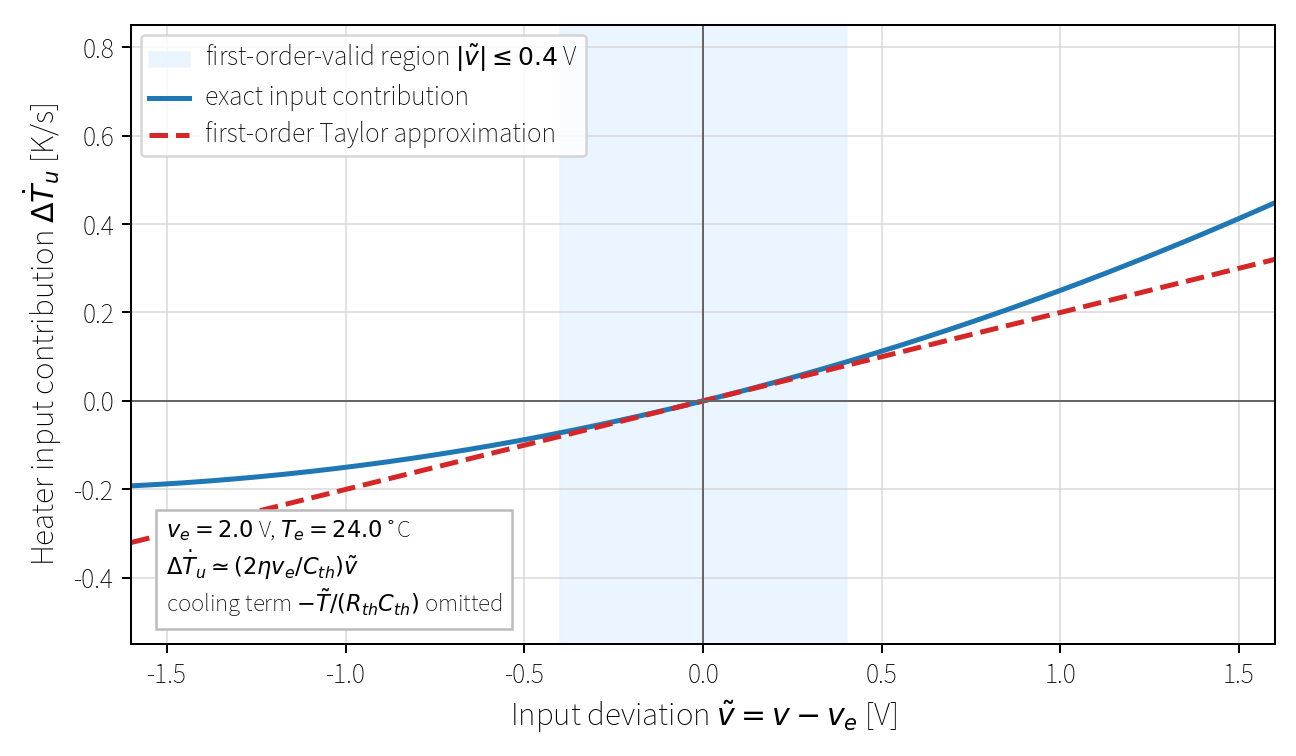
\includegraphics[width=0.86\linewidth,bb=0 0 1296 756]{figures/signal_modeling_linearization.png}
\caption{$T_a=20\,^\circ\mathrm{C}$、$R_{\mathrm{th}}=2.0\,\mathrm{K/W}$、$C_{\mathrm{th}}=10\,\mathrm{J/K}$、$\eta=0.5\,\mathrm{W/V^2}$、$v_e=2.0\,\mathrm{V}$ の動作点におけるヒータ入力寄与と一次 Taylor 近似。偏差が小さい範囲では一次近似を使いやすい。}
\label{fig:signal-modeling-linearization}
\end{figure}

\begin{figure}[tb]
\centering
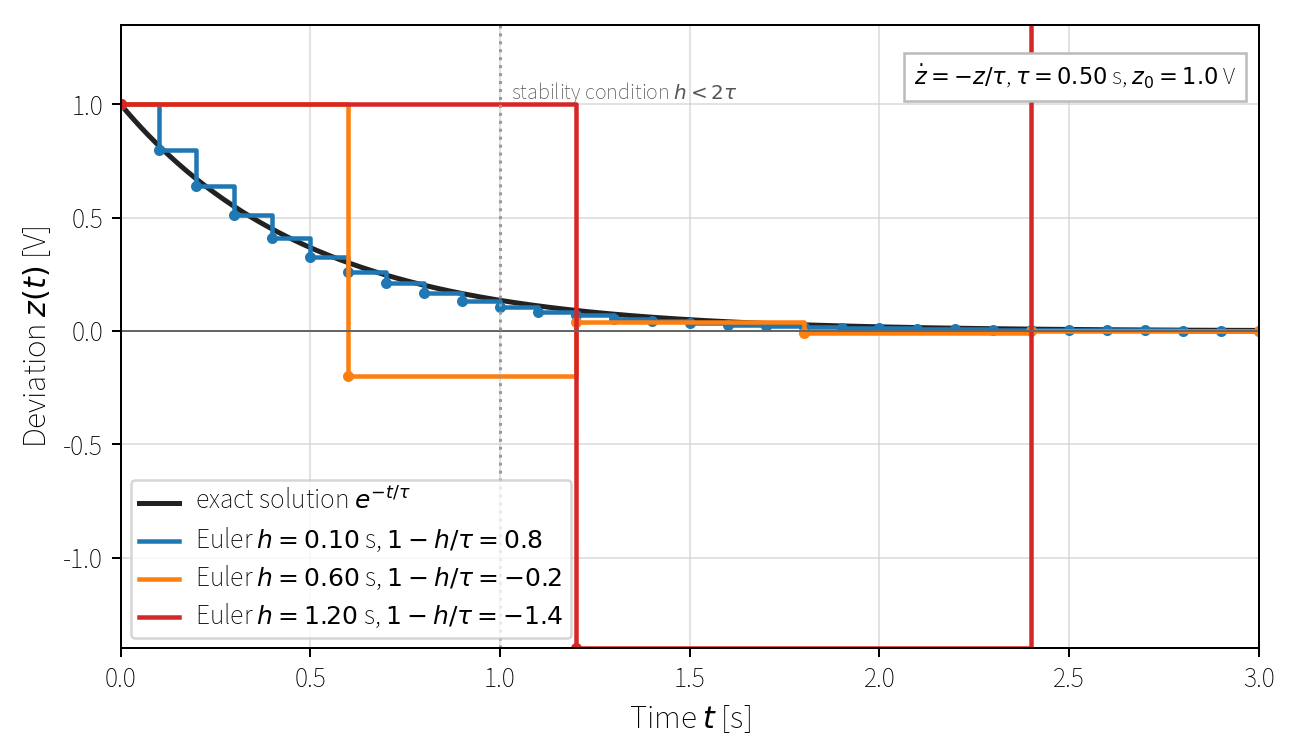
\includegraphics[width=0.86\linewidth,bb=0 0 1296 756]{figures/signal_modeling_euler_step.png}
\caption{$\dot{z}=-z/\tau$、$\tau=0.50\,\mathrm{s}$ に陽的 Euler 法を適用した応答。刻み幅 $h$ によって連続時間の減衰をどの程度再現できるかと、数値更新の安定性が変わる。}
\label{fig:signal-modeling-euler-step}
\end{figure}

\begin{practice}[信号分類と局所近似の確認]
図\ref{fig:signal-modeling-paths} で、対象の状態を直接変える信号と、センサ測定値だけを変える信号をそれぞれ列挙せよ。次に、図\ref{fig:signal-modeling-linearization} のパラメータから平衡温度 $T_e$ を計算し、$\tilde{v}=0.4\,\mathrm{V}$ と $\tilde{v}=1.2\,\mathrm{V}$ について、温度変化率へのヒータ入力寄与
\begin{equation}
  \frac{\eta\{(v_e+\tilde{v})^2-v_e^2\}}{C_{\mathrm{th}}},
  \qquad
  \frac{2\eta v_e}{C_{\mathrm{th}}}\tilde{v}
\end{equation}
を比較せよ。この二つの量は入力項だけの比較であり、完全な $\dot{\tilde{T}}$ には冷却項 $-\tilde{T}/(R_{\mathrm{th}}C_{\mathrm{th}})$ も加わることを確認せよ。さらに図\ref{fig:signal-modeling-euler-step} の $\tau=0.50\,\mathrm{s}$ について、$h=0.10\,\mathrm{s}$、$0.60\,\mathrm{s}$、$1.20\,\mathrm{s}$ の更新係数 $1-h/\tau$ を求め、連続時間の安定性と数値更新の安定性が一致しない場合を説明せよ。
\end{practice}

\subsubsection{標準例における信号の役割}

熱系では、部屋または小さな物体の代表温度を $T(t)$ [$^\circ\mathrm{C}$] とし、周囲温度を $T_a(t)$ [$^\circ\mathrm{C}$]、ヒータから実際に入る熱流を $u(t)$ [W] とする。熱容量 $C_{\mathrm{th}}$ [J/K] と熱抵抗 $R_{\mathrm{th}}$ [K/W] を一定パラメータとみなすと、単純なモデルは
\begin{equation}
  C_{\mathrm{th}}\dot{T}(t)
  =-\frac{T(t)-T_a(t)}{R_{\mathrm{th}}}+u(t)+d_q(t)
  \label{eq:thermal-signal-example}
\end{equation}
である。状態は $x=T$、入力はヒータ熱流 $u$、外乱は周囲温度 $T_a$ と未知熱流 $d_q$ である。制御したい出力を $y=T$、温度センサの測定値を $y_m=T+n_T$ と置けば、参照信号 $r=T_{\mathrm{ref}}$ は目標温度である。ここで $T_a$ は測れることも測れないこともある。測れる外乱はフィードフォワード補償に使えるが、測れない外乱はフィードバックで結果として抑える。

RC 回路では、コンデンサ電圧を $v_C(t)$ [V]、入力電圧を $u(t)=v_{\mathrm{in}}(t)$ [V]、外からコンデンサ節点へ流れ込む未知電流を $d_i(t)$ [A] とする。抵抗 $R$ [$\Omega$] と容量 $C$ [F] が一定なら、キルヒホッフの電流則から
\begin{equation}
  C\dot{v}_C(t)=\frac{u(t)-v_C(t)}{R}+d_i(t)
  \label{eq:rc-signal-example}
\end{equation}
を得る。$x=v_C$ とすれば、出力は $y=v_C$、センサ測定値は $y_m=v_C+n_v$ である。$R$ や $C$ は信号ではなくパラメータとして扱うが、温度による抵抗値変化を精密に扱う場合は、$R(t)$ をゆっくり変化する未知パラメータまたは追加状態として推定することがある。

質量ばねダンパ系では、位置 $q(t)$ [m]、速度 $\dot{q}(t)$ [m/s]、力入力 $u(t)$ [N]、外力外乱 $d_F(t)$ [N] を使う。質量 $M$ [kg]、粘性係数 $c$ [N\,s/m]、ばね定数 $k$ [N/m] を一定とすると、ニュートンの運動方程式は
\begin{equation}
  M\ddot{q}(t)+c\dot{q}(t)+kq(t)=u(t)+d_F(t)
  \label{eq:msd-signal-example}
\end{equation}
である。状態を
\begin{equation}
  x(t)=\begin{bmatrix}q(t)\\ \dot{q}(t)\end{bmatrix}
\end{equation}
と置くと
\begin{align}
  \dot{x}(t)&=
  \begin{bmatrix}
    0&1\\
    -k/M&-c/M
  \end{bmatrix}x(t)
  +\begin{bmatrix}0\\ 1/M\end{bmatrix}u(t)
  +\begin{bmatrix}0\\ 1/M\end{bmatrix}d_F(t),\label{eq:msd-state-signal-example}\\
  y(t)&=\begin{bmatrix}1&0\end{bmatrix}x(t),\\
  y_m(t)&=y(t)+n_q(t)
\end{align}
と書ける。位置センサしかない場合、測定量は位置 $q$ であり、センサ測定値は $q+n_q$ である。速度 $\dot{q}$ は状態の一部だが直接測れていないので、未測定状態である。後でオブザーバや Kalman フィルタを導入するのは、このような未測定状態を、入力と測定値の履歴から推定するためである。

DC モータなら、端子電圧 $v(t)$ [V] は入力、角速度 $\omega(t)$ [rad/s] や角度 $\theta(t)$ [rad] は出力になりうる。負荷トルク $\tau_L(t)$ [N\,m] は、制御器が直接選んでいないので外乱である。電機子インダクタンス $L$ [H]、抵抗 $R$ [$\Omega$]、逆起電力定数 $K_e$ [V\,s/rad]、トルク定数 $K_t$ [N\,m/A]、慣性モーメント $J$ [kg\,m$^2$]、粘性係数 $b$ [N\,m\,s/rad] を一定パラメータとすると、単純化したモデルは
\begin{align}
  L\dot{i}(t)&=-R i(t)-K_e\omega(t)+v(t),\label{eq:dc-motor-current}\\
  J\dot{\omega}(t)&=K_t i(t)-b\omega(t)-\tau_L(t),\label{eq:dc-motor-speed}\\
  \dot{\theta}(t)&=\omega(t).\label{eq:dc-motor-angle}
\end{align}
となる。

DC モータの端子電圧から角度までの関係は、代数的な直接変換ではなく、電気系と機械系の状態を通る因果連鎖として表される。電圧はまず電流を変化させ、電流がトルクを発生させ、トルクが角速度を変化させ、角速度の積分として角度が変化する。この因果連鎖を式の中に残すために、状態を導入する。

DC モータでは
\begin{equation}
  x(t)=\begin{bmatrix}i(t)\\ \omega(t)\\ \theta(t)\end{bmatrix}
\end{equation}
を状態にできる。状態 $x$、入力 $u$、外乱 $d$、パラメータ $p$、出力 $y$ を使うと、多くの対象は
\begin{align}
  \dot{x}(t)&=f(x(t),u(t),d(t),p,t),\label{eq:nonlinear-state-model}\\
  y(t)&=g(x(t),u(t),d(t),p,t)
\end{align}
と書ける。$f$ は内部がどう変わるか、$g$ はどの量が出力として取り出されるかを表す。

状態と出力は同じではない。状態は未来を計算するための内部記述であり、出力は目的やセンサ配置に応じて選ぶ見え方である。DC モータで角度制御をするなら $y=\theta$ と置くことが多いが、電流 $i$ と角速度 $\omega$ も未来の角度を決めるので状態に含める。電流センサがなければ $i$ は未測定状態であり、角度エンコーダがあれば $\theta+n_\theta$ がセンサ測定値である。状態フィードバックの章では $u=-Kx+r_u$ のように状態が使える場合を扱い、推定の章では測定値から $\hat{x}$ を作って、測れない状態を補う。
